\documentclass{ltjsarticle}

\usepackage{graphicx}
\usepackage{amsmath}
\usepackage{hyperref}
\usepackage{float}

\title{基礎PBL1 レポート}
\author{平野健汰}
\date{\today}

\begin{document}

\maketitle

\begin{abstract}
このレポートでは、チケット販売システムの設計に関する基本的な概念と手法について説明します。
\end{abstract}

\section{課題の説明}
スパイラル社はチケット販売業務を提供している.基本は電話対応である.このチケット販売業務のIT化を検討している.

クラウド社はソフトウェア開発会社でスパイラル社からチケット販売システムの開発を請け負うことになった.

今回の演習は,スパイラル社のチケット販売システムの設計を行うことである.

\section{要求分析}
\subsection{機能要件}
\begin{itemize}
  \item 必須要件
  \begin{itemize}
    \item サインアップ機能
    \item ログイン機能
    \item チケット検索機能
    \item チケット購入機能
    \item チケットを購入したことの証明書発行機能
  \end{itemize}
  \item 追加要件
  \begin{itemize}
    \item チケットの詳細表示機能
    \item 支払方法選択機能
    \item クレジットカード決済機能
    \item コンビニ決済機能
    \item 電子マネー決済機能
    \item 仮想通貨決済機能
    \item クレジットカード照会機能
    \item チケット購入履歴表示機能
  \end{itemize}
\end{itemize}

\subsection{GUI紙芝居}
\begin{figure}
    \centering
    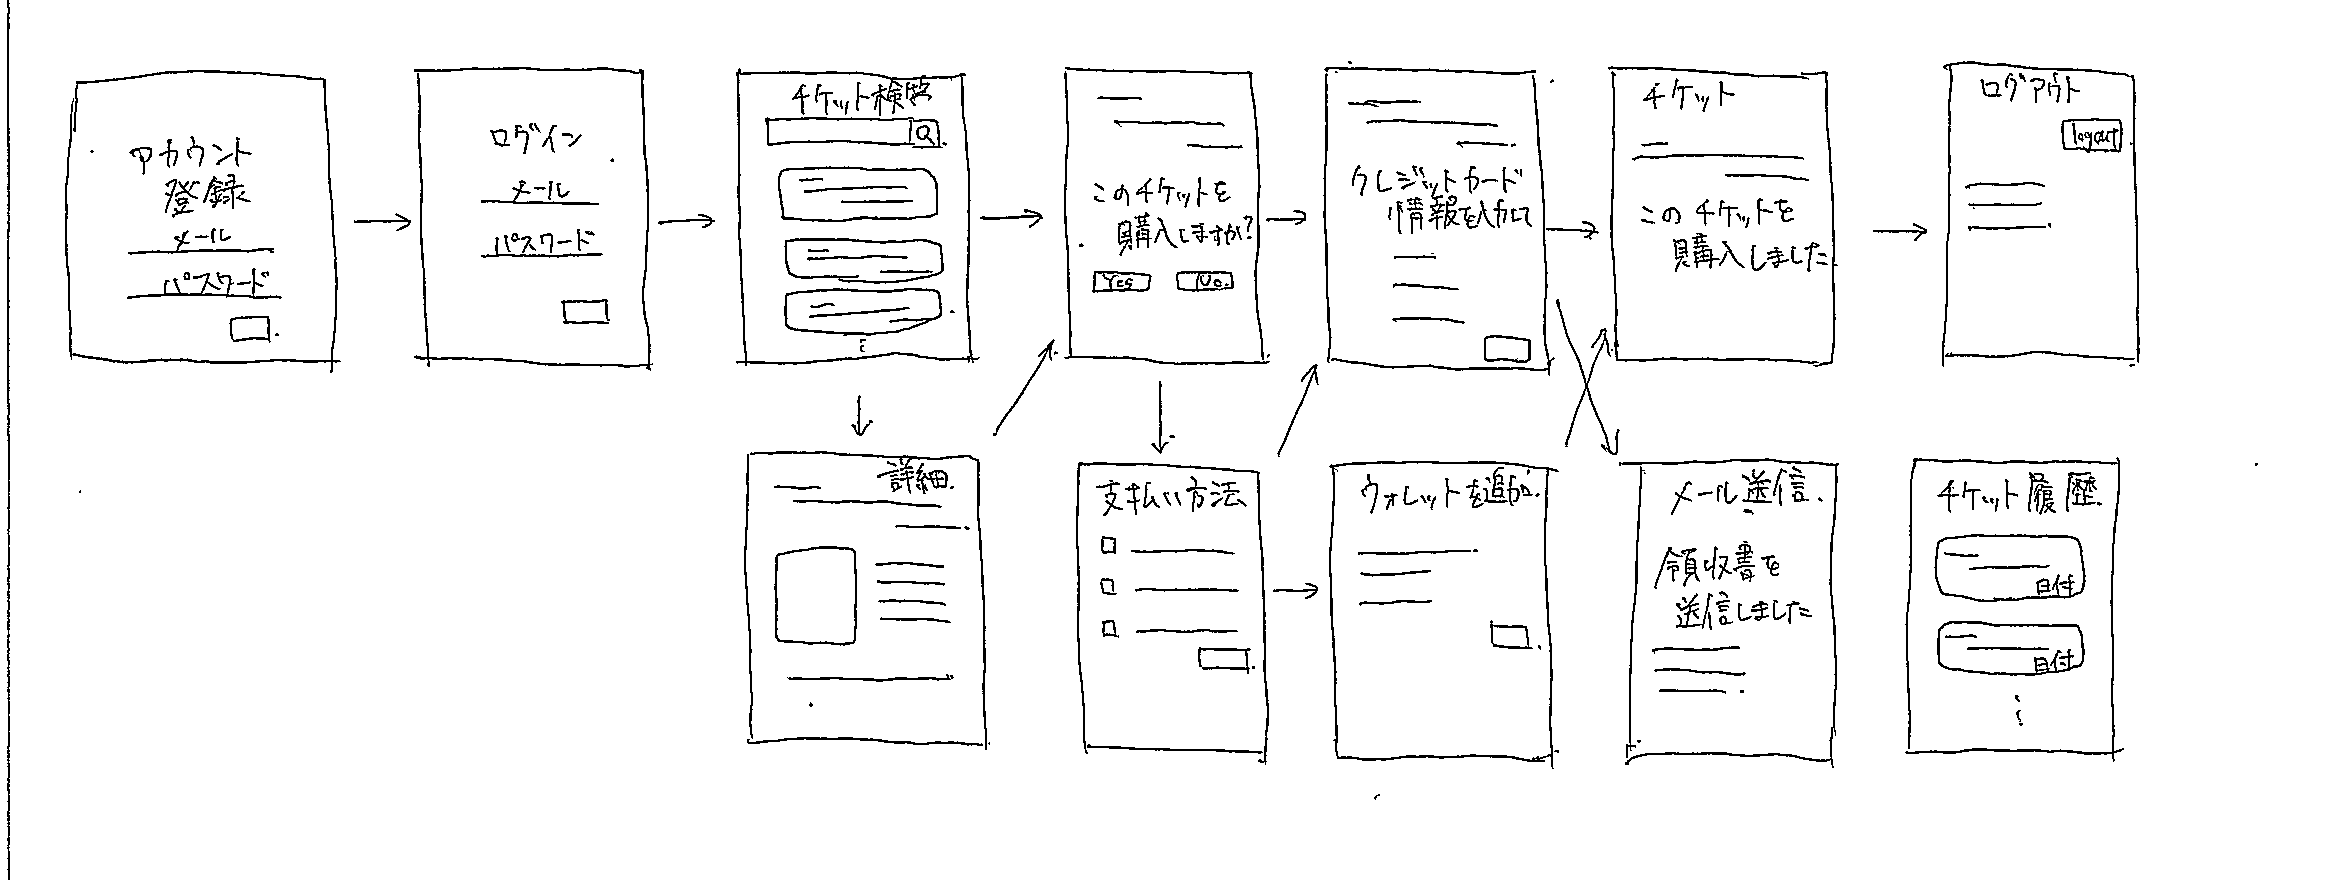
\includegraphics[width=0.8\textwidth]{src/GUI.png}
    \caption{GUI紙芝居}
    \label{fig:gui}
\end{figure}

\subsection{ドメインモデル図}
今回作成したドメインモデル図は以下のとおりである.
\begin{figure}[H]
    \centering
    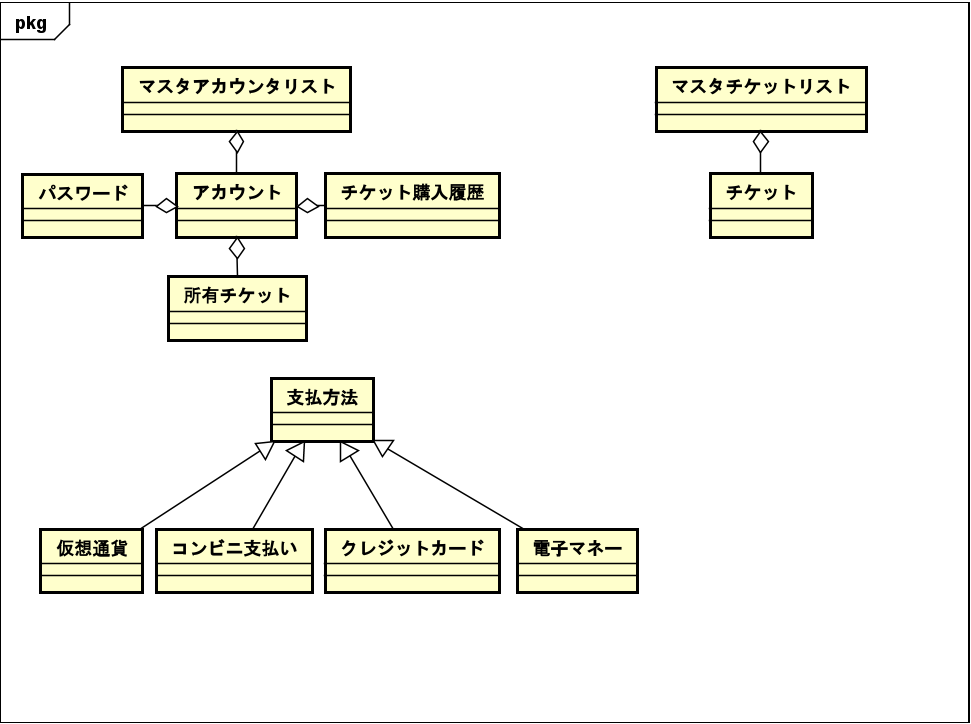
\includegraphics[width=0.8\textwidth]{src/DomainModel.png}
    \caption{ドメインモデル図}
    \label{fig:domain_model}
\end{figure}

以上が今回作成したドメインモデル図であるが,この図の説明を簡単に記述する.
ドメインモデル図の目的は,ドメインの構造を理解することである.具体的には,ドメインの構造を理解し,ドメインの概念を明確にすることである.
この図は集約と汎化が含まれている.集約は全体と個の関係を持っている.汎化は抽象と具体の関係を持っている.
具体的には以下のとおりである.
\begin{figure}[H]
    \centering
    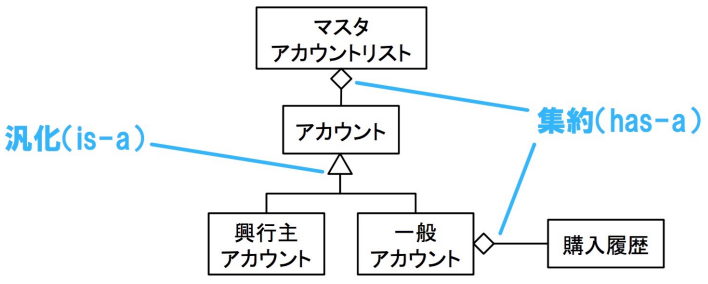
\includegraphics[width=0.8\textwidth]{src/ExampleDomainModel.png}
    \caption{ドメインモデル図}
    \label{fig:domain_model2}
\end{figure}

\subsection{ユースケース図}
今回作成したユースケース図は以下のとおりである.
\begin{figure}[H]
    \centering
    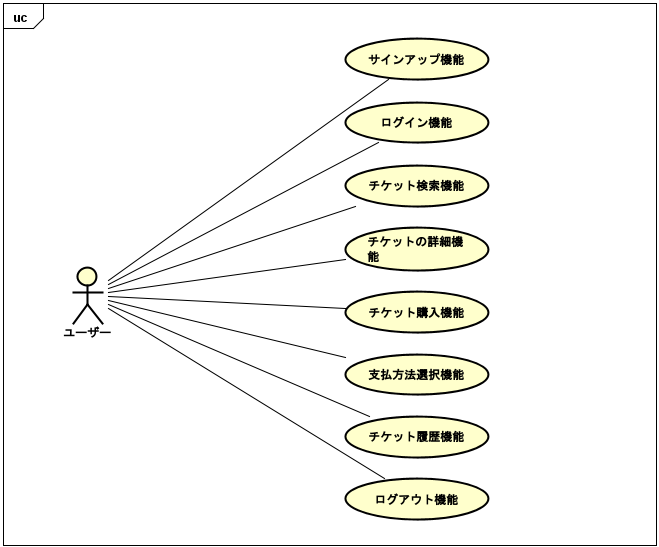
\includegraphics[width=0.8\textwidth]{src/Usecase.png}
    \caption{ユースケース図}
    \label{fig:use_case}
\end{figure}

以上が今回作成したユースケース図であるが,この図の説明を簡単に記述する.
ユースケース図の目的は,システムのふるまいを理解することである.具体的には,システムの機能を理解し,システムの機能を明確にすることである.
この図はアクタとユースケースが含まれている.アクタは実際に行動を起こす人のことで今回の場合はユーザである.ユースケースは実際にアクタができることである.
図を利用して説明すると以下のとおりである.

\begin{figure}[H]
    \centering
    \includegraphics[width=0.8\textwidth]{src/ExampleUsecase.png}
    \caption{ユースケース図}
    \label{fig:use_case2}
\end{figure}

\subsection{ユースケース記述}
今回作成したユースケース記述について以下に記述する.
\subsubsection{ログイン機能}
\begin{itemize}
    \item ユースケース名: ログイン
    \item アクター: ユーザ
    \item 前提条件: ユーザがアプリケーションにアクセスしている
    \item 事後条件: ユーザがログインしている
    \item 基本フロー:
    \begin{enumerate}
        \item ユーザがログイン画面にアクセスする
        \item ユーザがユーザ名とパスワードを入力する
        \item システムがユーザ名とパスワードを検証する
        \item システムがユーザをログイン状態にする
    \end{enumerate}
    \item 代替フロー:
    \begin{enumerate}
        \item ユーザがユーザ名とパスワードを間違えた場合
        \begin{enumerate}
            \item システムがエラーメッセージを表示する
            \item ユーザが再度ユーザ名とパスワードを入力する
        \end{enumerate}
    \end{enumerate}
\end{itemize}

\subsubsection{チケット検索機能}
\begin{itemize}
    \item ユースケース名: チケット検索
    \item アクター: ユーザ
    \item 前提条件: ユーザがログインしている
    \item 事後条件: ユーザがチケットを検索している
    \item 基本フロー:
    \begin{enumerate}
        \item ユーザがチケット検索画面にアクセスする
        \item ユーザが検索条件を入力する
        \item システムが検索条件に一致するチケットを表示する
    \end{enumerate}
    \item 代替フロー:
    \begin{enumerate}
        \item ユーザが検索条件を入力しなかった場合
        \begin{enumerate}
            \item システムが全てのチケットを表示する
        \end{enumerate}
    \end{enumerate}
\end{itemize}

ユースケース記述の目的は各ユースケースの具体化・詳細化である.

\section{オブジェクト指向分析/設計}
\subsection{ロバストネス図の作成}
今回作成したロバストネス図は以下のとおりである.
\subsubsection{ログイン機能}
\begin{figure}[H]
    \centering
    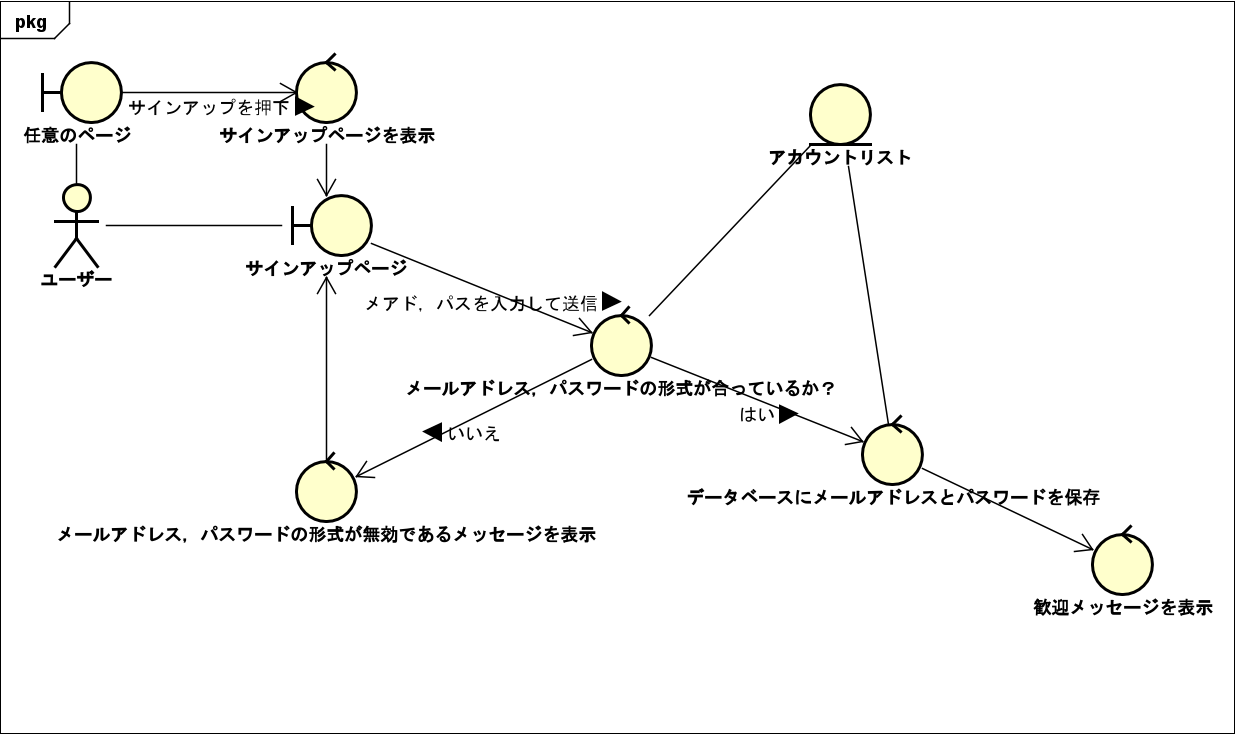
\includegraphics[width=0.8\textwidth]{src/Robustness.png}
    \caption{ロバストネス図}
    \label{fig:robustness}
\end{figure}

\subsubsection{チケット検索機能}
\begin{figure}[H]
    \centering
    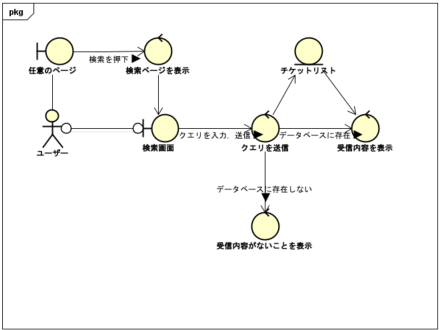
\includegraphics[width=0.8\textwidth]{src/Robustness2.png}
    \caption{ロバストネス図}
    \label{fig:robustness2}
\end{figure}

以上が今回作成したロバストネス図であるが,この図の説明を簡単に記述する.
ロバストネス図の目的はUC記述の洗練である.具体的には,UC記述の可視化,分析しその妥当性を確認することである.

この図にはステレオタイプが3つ含まれている.
具体的には以下のとおりである.
\begin{figure}[H]
    \centering
    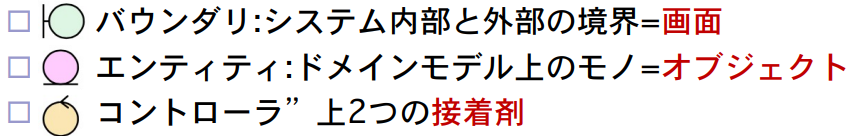
\includegraphics[width=0.8\textwidth]{src/ExampleRobustness.png}
    \caption{ロバストネス図}
    \label{fig:robustness2}
\end{figure}

\subsection{シーケンス図の作成}
今回作成したシーケンス図は以下のとおりである.
\subsubsection{ログインシーケンス}
\begin{figure}[H]
    \centering
    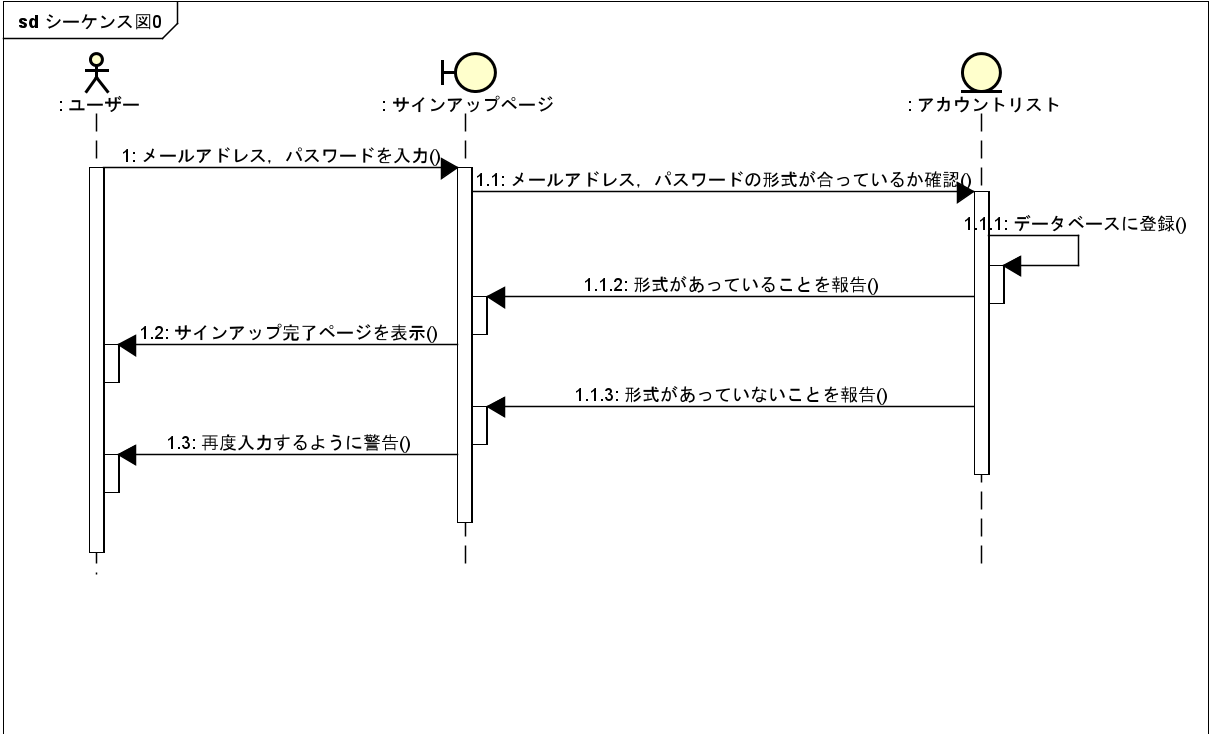
\includegraphics[width=0.8\textwidth]{src/Sequence.png}
    \caption{シーケンス図}
    \label{fig:sequence}
\end{figure}

\subsubsection{チケット検索シーケンス}
\begin{figure}[H]
    \centering
    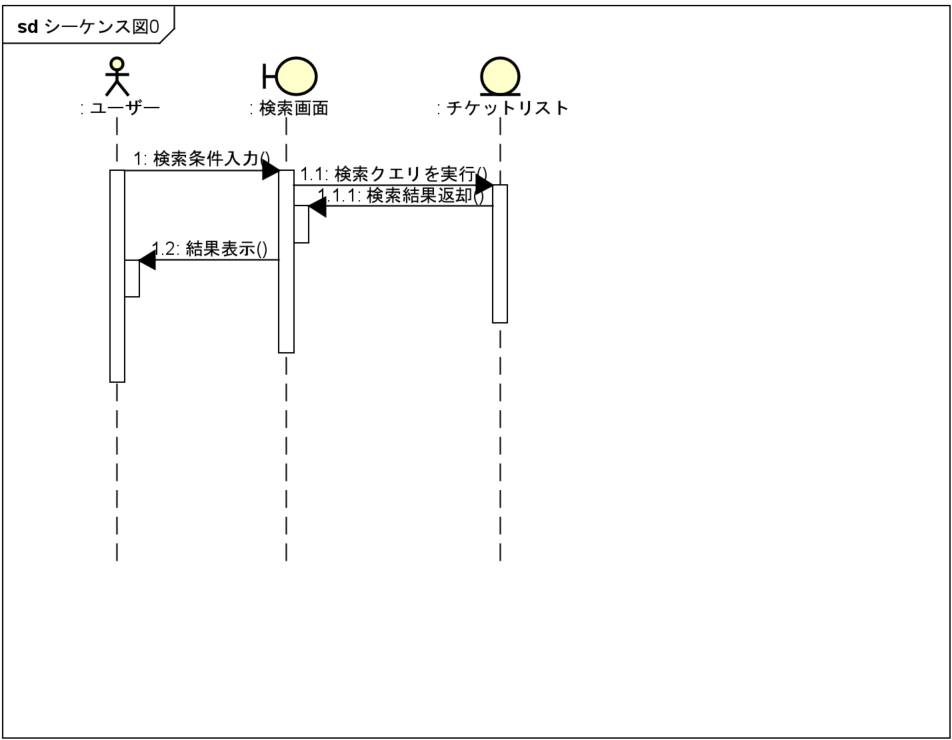
\includegraphics[width=0.8\textwidth]{src/Sequence2.png}
    \caption{シーケンス図}
    \label{fig:sequence2}
\end{figure}

以上が今回作成したシーケンス図であるが,この図の説明を簡単に記述する.
シーケンス図の目的はクラスの責務割り当てである.具体的には,クラスの責務を明確にし,クラス間の協調を明確にすることである.

この図はロバストネス図を基にバウンダリとエンティティをクラスに変換しコントローラを矢印に置き換えたものである.

\subsection{クラス図の作成}
今回作成したクラス図は以下のとおりである.
\subsubsection{ログインクラス}
\begin{figure}[H]
    \centering
    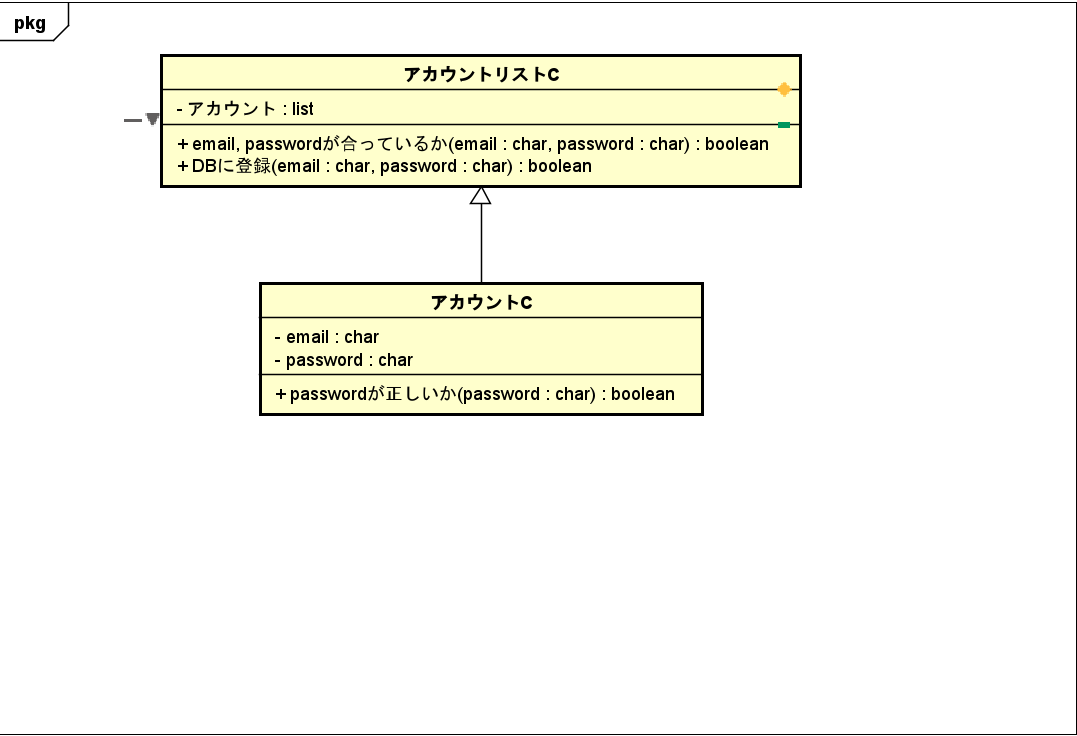
\includegraphics[width=0.8\textwidth]{src/Class.png}
    \caption{クラス図}
    \label{fig:class}
\end{figure}

\subsubsection{チケット検索クラス}
\begin{figure}[H]
    \centering
    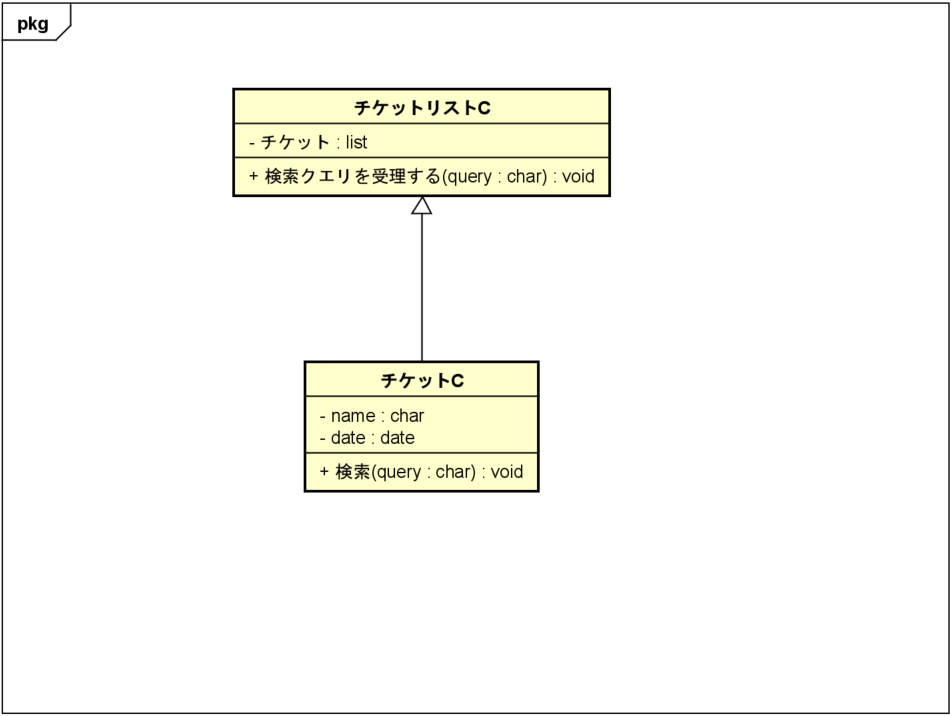
\includegraphics[width=0.8\textwidth]{src/Class2.png}
    \caption{クラス図}
    \label{fig:class2}
\end{figure}

以上が今回作成したクラス図であるが,この図の説明を簡単に記述する.
クラス図の目的はクラスの責務を構造化することである.具体的には,クラスの属性とふるまいを構造化することである.

クラス図はシーケンス図を基に作成することができる.
クラス図はクラス名,属性,ふるまいを記述する.
具体的なクラス図の説明は以下のとおりである.
\begin{figure}[H]
    \centering
    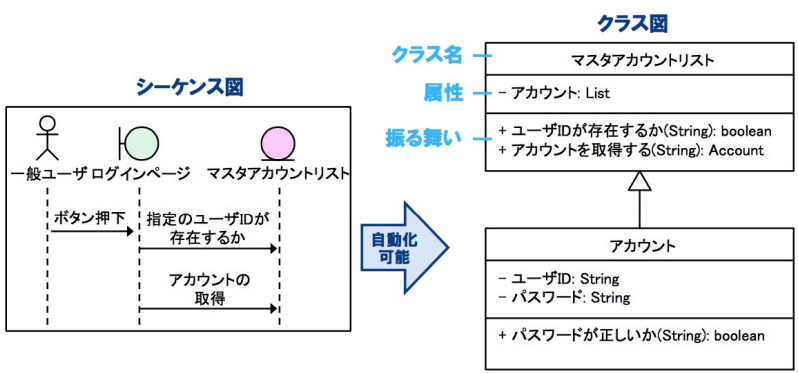
\includegraphics[width=0.8\textwidth]{src/ExampleClass.png}
    \caption{クラス図}
    \label{fig:class2}
\end{figure}


\section{考察}
今回の演習を通して,チケット販売システムの設計に関する基本的な概念と手法を学ぶことができた.今回,要件定義から,ドメインモデル図,ユースケース図,ロバストネス図,シーケンス図,クラス図を作成することで,システムの設計について理解を深めることができた.

今回の演習を通じて,初めはユーザー側の視点から要件定義を行い,それらをドメインモデル図,ユースケース図を利用して図式化し,抽象化した.その後,それぞれのユースケースを記述することで具体化していき,ロバストネス図,シーケンス図,クラス図を作成することでシステムを構造化して確認することができる.
つまり,初めは具体的なことから考え,抽象化し,それらを細分化して,再び具体化することでシステムの設計を行うことができると考えた.

\end{document}